\poczatekwykladu{4}
\section{Generatory sigma-ciała borelowskiego}
\label{sec:generatory-borelowskie}

Niech $\mathcal{J}$ oznacza rodzinę wszystkich przedziałów w $\R$,
z dopuszczeniem przedziałów nieograniczonych i zbioru pustego.
Sigma-ciało borelowskie na prostej oznaczamy również przez
$\mathcal{B}_{\R}$ lub $\operatorname{Bor}(\R)$.
Rozważmy rodziny
\begin{align*}
  \mathcal{J}_0&=\{(a,b):a,b\in\R,\ a<b\},\\
  \mathcal{J}_D&=\{[a,b]:a,b\in\R,\ a\leq b\},\\
  \mathcal{J}_P&=\{(a,b]:a,b\in\R,\ a<b\},\\
  \mathcal{P}_0^-&=\{(-\infty,b):b\in\R\},
  &\mathcal{P}_D^-&=\{(-\infty,b]:b\in\R\},\\
  \mathcal{P}_0^+&=\{(a,+\infty):a\in\R\},
  &\mathcal{P}_D^+&=\{[a,+\infty):a\in\R\}.
\end{align*}

\begin{twierdzenie}[Generatory sigma-ciała borelowskiego na prostej]
\label{tw:generatory-borelowskie}
Zachodzą równości
\begin{equation}
  \begin{aligned}
    \mathcal{B}(\R)
      &=\sigma(\mathcal{J})=\sigma(\mathcal{J}_0)\\
      &=\sigma(\mathcal{J}_D)=\sigma(\mathcal{J}_P)\\
      &=\sigma(\mathcal{P}_0^-)=\sigma(\mathcal{P}_D^-)\\
      &=\sigma(\mathcal{P}_0^+)=\sigma(\mathcal{P}_D^+).
  \end{aligned}
  \label{eq:generatory-borelowskie}
\end{equation}
\end{twierdzenie}

Do dowodu wykorzystamy dwie własności operacji generowania sigma-ciała.

\begin{lemat}[Monotoniczność generowania]
\label{lem:monotonicznosc-generowania}
Jeżeli $\mathcal{E}\subseteq\mathcal{E}'\subseteq\mathcal{P}(X)$, to
\[
  \sigma(\mathcal{E})\subseteq\sigma(\mathcal{E}').
\]
\end{lemat}

\begin{proof}
Sigma-ciało $\sigma(\mathcal{E}')$ zawiera $\mathcal{E}'$, więc zawiera
także $\mathcal{E}$. Ponieważ $\sigma(\mathcal{E})$ jest najmniejszym
sigma-ciałem zawierającym $\mathcal{E}$, otrzymujemy żądaną inkluzję.
\end{proof}

\begin{wniosek}[Idempotentność generowania]
\label{wn:idempotentnosc-generowania}
Dla każdej rodziny $\mathcal{E}\subseteq\mathcal{P}(X)$ mamy
\[
  \sigma\bigl(\sigma(\mathcal{E})\bigr)=\sigma(\mathcal{E}).
\]
\end{wniosek}

\begin{proof}
Rodzina $\sigma(\mathcal{E})$ jest już sigma-ciałem, więc jest
najmniejszym sigma-ciałem zawierającym samą siebie.
\end{proof}

\begin{proof}[Dowód twierdzenia~\ref{tw:generatory-borelowskie}]
\emph{Przedziały otwarte i wszystkie przedziały.}
Równość $\mathcal{B}(\R)=\sigma(\mathcal{J}_0)$ została uzasadniona
w \eqref{eq:borel-odcinki}. Ponieważ $\mathcal{J}_0\subseteq\mathcal{J}$,
lemat~\ref{lem:monotonicznosc-generowania} daje
$\sigma(\mathcal{J}_0)\subseteq\sigma(\mathcal{J})$.
Z drugiej strony dla $a\leq b$ mamy
\begin{equation}
  [a,b]=\bigcap_{n=1}^{\infty}
    \left(a-\frac1n,b+\frac1n\right),
  \label{eq:przedzial-domkniety-przekroj}
\end{equation}
a dla $a<b$ również
\begin{align*}
  [a,b)&=\bigcap_{n=1}^{\infty}\left(a-\frac1n,b\right),\\
  (a,b]&=\bigcap_{n=1}^{\infty}\left(a,b+\frac1n\right).
\end{align*}
Wszystkie te zbiory należą do $\sigma(\mathcal{J}_0)$.
Przedziały nieograniczone otrzymujemy jako przeliczalne sumy
przedziałów ograniczonych tego samego typu.
Ponadto $\R=\bigcup_{n=1}^{\infty}(-n,n)$, a zbiór pusty należy
do każdego sigma-ciała. Zatem $\mathcal{J}\subseteq\sigma(\mathcal{J}_0)$,
co daje
\[
  \sigma(\mathcal{J})\subseteq
  \sigma\bigl(\sigma(\mathcal{J}_0)\bigr)
  =\sigma(\mathcal{J}_0)=\mathcal{B}(\R).
\]

\begin{figure}[htbp]
  \centering
  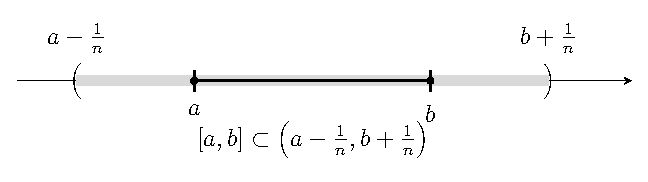
\includegraphics[width=0.82\textwidth]{aproksymacja-przedzialu.pdf}
  \caption{Przedział domknięty jako przekrój malejących przedziałów otwartych.}
  \label{fig:aproksymacja-przedzialu}
\end{figure}

\emph{Przedziały domknięte.}
Z inkluzji $\mathcal{J}_D\subseteq\mathcal{J}$ wynika
$\sigma(\mathcal{J}_D)\subseteq\mathcal{B}(\R)$.
Dla $a<b$ wybierzmy $n_0\in\N$ tak duże, aby $2/n_0<b-a$.
Wówczas
\begin{equation}
  (a,b)=\bigcup_{n=n_0}^{\infty}
    \left[a+\frac1n,b-\frac1n\right]
  \in\sigma(\mathcal{J}_D).
  \label{eq:przedzial-otwarty-suma-domknietych}
\end{equation}
Można też skorzystać z równości
\[
  (a,b)=[a,b]\setminus\bigl(\{a\}\cup\{b\}\bigr),
  \qquad \{a\}=[a,a],\quad\{b\}=[b,b].
\]
Stąd $\mathcal{J}_0\subseteq\sigma(\mathcal{J}_D)$, a więc
$\mathcal{B}(\R)\subseteq\sigma(\mathcal{J}_D)$.

\emph{Przedziały półotwarte.}
Inkluzja $\mathcal{J}_P\subseteq\mathcal{J}$ daje
$\sigma(\mathcal{J}_P)\subseteq\mathcal{B}(\R)$.
Dla $a<b$ i dostatecznie dużego $n_0$ mamy
\[
  (a,b)=\bigcup_{n=n_0}^{\infty}
    \left(a,b-\frac1n\right]\in\sigma(\mathcal{J}_P).
\]
Otrzymujemy przeciwną inkluzję, zatem
$\sigma(\mathcal{J}_P)=\mathcal{B}(\R)$.

\emph{Półproste otwarte.}
Każda półprosta $(-\infty,b)$ należy do $\mathcal{B}(\R)$, ponieważ
\[
  (-\infty,b)=\bigcup_{n=n_0}^{\infty}(-n,b)
\]
dla $n_0$ tak dużego, aby $-n_0<b$.
Stąd $\sigma(\mathcal{P}_0^-)\subseteq\mathcal{B}(\R)$.
Aby uzyskać przeciwną inkluzję, zauważmy, że
\[
  (a,+\infty)=(-\infty,a]^c
    =\left(\bigcap_{n=1}^{\infty}
      \left(-\infty,a+\frac1n\right)\right)^c
    \in\sigma(\mathcal{P}_0^-).
\]
Zatem
\[
  (a,b)=(-\infty,b)\cap(a,+\infty)
    \in\sigma(\mathcal{P}_0^-).
\]
To daje $\mathcal{J}_0\subseteq\sigma(\mathcal{P}_0^-)$ i w konsekwencji
$\mathcal{B}(\R)=\sigma(\mathcal{P}_0^-)$.
Analogicznie dla prawych półprostych korzystamy z równości
\[
  (-\infty,b)=
    \left(\bigcap_{n=1}^{\infty}
      \left(b-\frac1n,+\infty\right)\right)^c
\]
oraz $(a,b)=(a,+\infty)\cap(-\infty,b)$.
Otrzymujemy $\mathcal{B}(\R)=\sigma(\mathcal{P}_0^+)$.

\emph{Półproste domknięte.}
Pozostałe równości wynikają w ten sam sposób z zależności
\begin{align*}
  (-\infty,b]&=\bigcap_{n=1}^{\infty}
    \left(-\infty,b+\frac1n\right),
  &(-\infty,b)&=\bigcup_{n=1}^{\infty}
    \left(-\infty,b-\frac1n\right],\\
  [a,+\infty)&=\bigcap_{n=1}^{\infty}
    \left(a-\frac1n,+\infty\right),
  &(a,+\infty)&=\bigcup_{n=1}^{\infty}
    \left[a+\frac1n,+\infty\right).
\end{align*}
Rodziny półprostych otwartych i domkniętych generują więc te same sigma-ciała.
\end{proof}

\begin{uwaga}[Zbiory borelowskie w $\R^d$]
W przestrzeni $\R^d$ można zdefiniować sigma-ciało borelowskie jako
sigma-ciało generowane przez prostokąty
\[
  I_1\times\cdots\times I_d,
\]
gdzie $I_1,\ldots,I_d$ są przedziałami w $\R$.
\end{uwaga}

\section{Zbiory otwarte i sigma-ciało borelowskie}
\label{sec:otwarte-borelowskie}

\begin{definicja}[Zbiór otwarty na prostej]
Zbiór $U\subseteq\R$ nazywamy otwartym, jeżeli
\[
  \forall x\in U\ \exists\delta>0\qquad (x-\delta,x+\delta)\subseteq U.
\]
\end{definicja}

\begin{figure}[htbp]
  \centering
  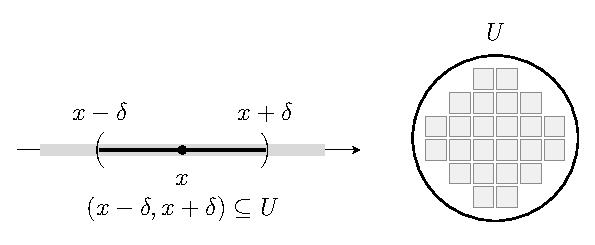
\includegraphics[width=0.91\textwidth]{otoczenie-punktu.pdf}
  \caption{Otoczenie punktu zbioru otwartego oraz prostokąty wewnątrz koła.}
  \label{fig:otoczenie-punktu}
\end{figure}

\begin{twierdzenie}
\label{tw:borelowskie-otwarte}
Niech $\tau$ będzie rodziną wszystkich zbiorów otwartych w $\R$.
Wówczas
\[
  \mathcal{B}(\R)=\sigma(\tau).
\]
\end{twierdzenie}

\begin{proof}
Każdy przedział otwarty jest zbiorem otwartym, więc
$\mathcal{B}(\R)=\sigma(\mathcal{J}_0)\subseteq\sigma(\tau)$.
Z drugiej strony każdy zbiór otwarty $U$ jest sumą zawartych w nim
przedziałów o wymiernych końcach. Jest ich co najwyżej przeliczalnie wiele,
jak w dowodzie \eqref{eq:borel-odcinki}. Zatem $\tau\subseteq\mathcal{B}(\R)$,
co daje przeciwną inkluzję.
\end{proof}

\begin{uwaga}
W przestrzeniach metrycznych, a ogólniej topologicznych, sigma-ciało
borelowskie definiuje się jako sigma-ciało generowane przez zbiory otwarte.
\end{uwaga}
